The main focus of studying dynamical systems is to understand the possible states an observable solution can experience and with most engineering, physics or even chemical systems, this is a cumbersome task. This approach allows for conditions to be given for when a solution can be found or when it has stable behavior. Often we find parameters inherent in the model for the system to play huge roles in the dynamical behavior and can be the difference between a system being capable of finding an equilibrium or not. When we find a parameter that has this effect, we call it a bifurcation parameter as there is some value that can be found that suddenly bifurcates the behavior of the system. The canonical example and one of the first to be studied was the system that contained a saddle-node bifurcation

\begin{equation}\label{eq:intro_saddlenode}
\dot{x}=a-x^2.
\end{equation}

\begin{figure}[H]
\centering
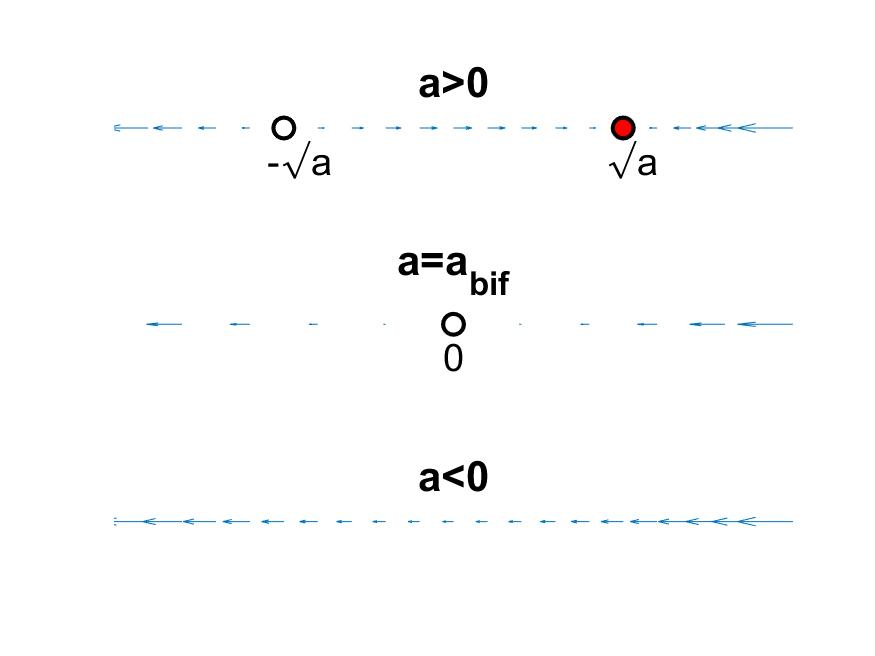
\includegraphics[width=\linewidth]{intro/saddlenode.jpg}
\caption{Vector field of a saddle-node bifurcation}
\label{fig:intro_saddlenode}
\end{figure}


\begin{figure}[H]
\centering
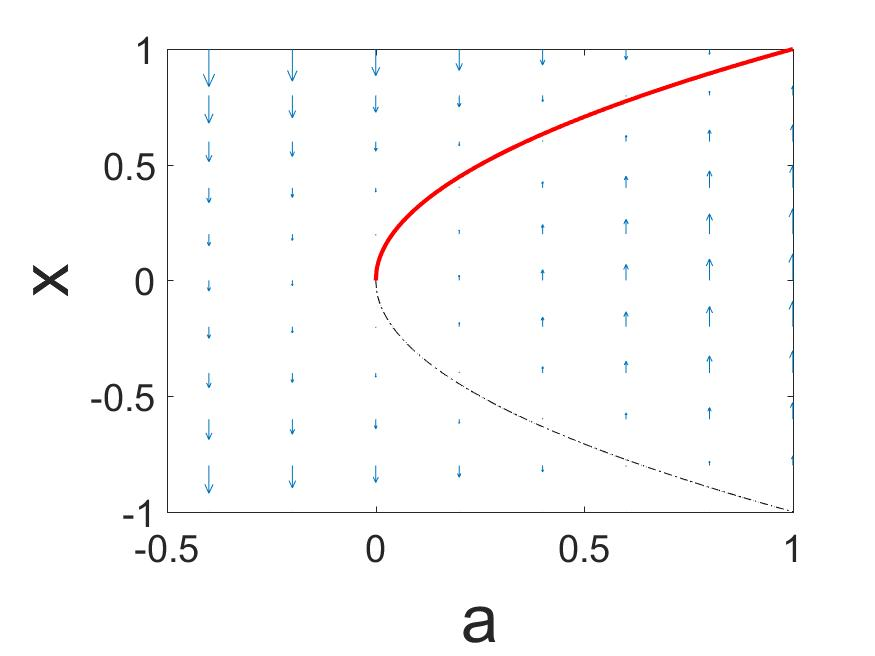
\includegraphics[width=.7\linewidth]{intro/saddlenode_bif_diagram.jpg}
\caption{Diagram of saddle-node bifurcation}
\label{fig:intro_saddlenode_bif_diagram}
\end{figure}



In figure~\ref{fig:intro_saddlenode} we show the vector field of the system that contains a saddle-node bifurcation. The equilibrium of this system is $x=\pm \sqrt{a}$ for any $a>0$ where stable equilibrium points with solid lines and unstable with dash-dotted lines. Notice that at $a=0$ and when $a<0$ we are no longer unable to find a stable equilibrium. This is known to be the simplest example of different qualitative behavior arising from a change in the parameter and it happens by two equilibria annihilating. In figure~\ref{fig:intro_saddlenode_bif_diagram} we plot the same system against the parameter $a$, which we call the phase plane. Here we still see the region with two equilibrium, the bifurcation and the region of no stability. Although, there are many types of bifurcations that have arisen in different systems that each have their own key properties. Studying these properties lead to a deeper understanding of the system on both the global and local scale. Much work has been done on systems that have smooth bifurcations due to the analysis being easier to perform, but non-smooth dynamics still are present in the physical world.

Non-smooth bifurcations are a topic that arise in special systems and for how frequent they appear, they have not been studied nearly as much as their smooth counter parts. This paper discusses the role of the non-smooth saddle-node bifurcation in a simplified one-dimensional system in \autoref{chap:oneD} as well as in the classic two-dimensional Stommel model for Thermohalcine current dynamics in \autoref{chap:twoD}. But many interesting ocean and weather mechanisms may be incorporated into the Stommel model to provide more realistic predictions for weather patterns. We choose to study slowly varying bifurcation parameters and their effect on the stability of a system while contrasting this with non-autonomous oscillatory forcing. The interaction of these features create complex dynamics around the standard bifurcations and can lead to early bifurcation or delayed tipping. For the one-dimensional system, a detailed analysis of these features is done on the smooth bifurcation in \cite{zhu2015tipping}.

\section*{Stommel Model}

Global circulation models have primarily focused on three different categories: 
\begin{itemize}
\item Atmospheric- the effect of greenhouse gases have on the atmosphere,
\item Oceanic- the effect of tides and interaction of temperature with salinity in the ocean,
\item Sea ice and land surface components.
\end{itemize}
These categories all contribute significantly to the overall prediction of weather and climate for the planet, which has importance to just about every industry and economy. Failure to adhere to and prepare for sudden changes in the climate led to drastic situations like severe droughts or ocean acidification. Atmospheric models have been vastly studied but far less work has been done on the contribution from the ocean and the dynamics that drive the tides and current.

A key feature of oceanic contributions is when patterns form around regions of bi-stability of temperature and salinity. An example of this is the thermohaline circulation (THC) which experience abrupt qualitative changes at certain points, see \cite{alley2003abrupt,marotzke2000abrupt,rahmstorf2000thermohaline,rahmstorf2002ocean}. Just earlier this year evidence was found of weakening occurring around these abrupt changes in a system of ocean patterns known as the Atlantic meridional overturning circulation (AMOC) \cite{caesar2018AMOC}. This is the first evidence of ocean dynamics responding to temperature change on the surface and can help further predict the future of the system. It is imperative that appropriate action is taken to prepare for the future of these type of systems as they are outside our realm of control. 

To study these phenomenon we create parametric models to replicate the dynamics we observe. Initially, Henry Stommel proposed the two box model in 1961 to understand the physics of the THC, shown in figure~\ref{fig:stommel_boxes}. In \cite{stommel1961thermohaline}, it is suggested that there are actually two different stability regimes which even overlap in the system that is proposed and concluded that oceanic dynamics behave very similarly about these equilibria. These type of systems have since been a heavily studied area for both climatology due to the wide ranging applications and dynamical systems for its generalization into dual stability.

\begin{figure}[H]
\centering
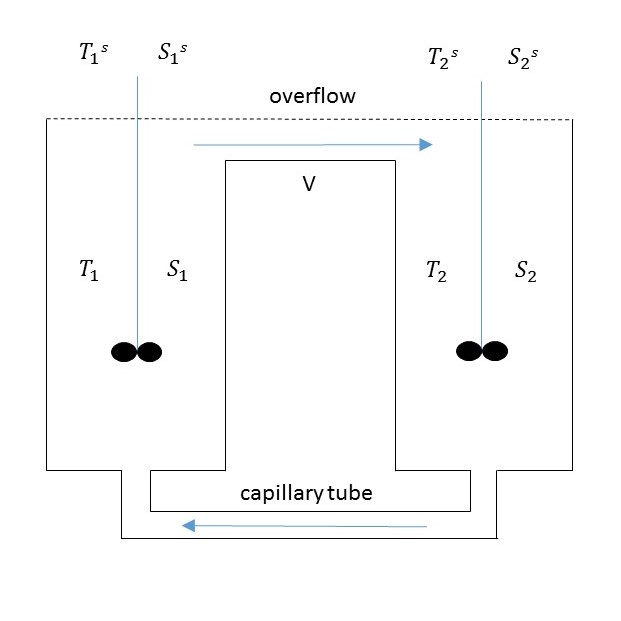
\includegraphics[width=0.7\textwidth]{intro/box.jpg}
\caption{The Stommel Two Box Model: Differing volume boxes with a temperature and salinity, $T_i$ and $S_i$. The boxes are connected by an overflow and capillary tube that has a flow $V$. There is also a surface temperature and salinity for each box, ${T_i}^s$ and ${S_i}^s$. We assume that there is some stirring to give a well mixed structure.}
\label{fig:stommel_boxes}
\end{figure}

With emphasis on mathematics, the focus of this paper is on developing an effective approach to problems with bi-stability and additional mechanisms and thus the physical quantities are brushed aside in favor of their non-dimensional alternatives. The non-dimensionalized Stommel Model is represented with the system

\begin{equation}
 \begin{aligned}
  \dot{T} & = \eta_1-T(1+|T-S|), \\
  \dot{S}   & = \eta_2-S(\eta_3+|T-S|). 
 \end{aligned}
\end{equation}

The variables $T$ and $S$ are the temperature and salinity respectively, the parameters $\eta_1$, $\eta_2$, and $\eta_3$ are all dimensionless quantities that all have physical interpretation to the relaxation times and volumes of the box. Where $\eta_1$ is thought of as the thermal variation, $\eta_2$ as the saline variation otherwise known as the freshwater flux, and $\eta_3$ as the ratio of relaxation times of temperature and salinity. Here $\eta_1$ is a positive quantity that takes any value whereas $\eta_3$ is also positive but has the property to determine the orientation of the equilibria. A standard orientation will be when $\eta_3<1$, $\eta_3=1$ is a special case and $\eta_3>1$ will have reverse orientation, this is seen in figure~\ref{fig:Stommel_bif_plots}. This is due to the nature of the parameter, when $\eta_3=1$, the relaxation rates for both the thermal and salinity variables are the same and hence we lose the dual stability.

The parameter $\eta_2$ is the most interesting as different values cause major qualitative and quantitative changes in the dynamics of the system. These changes have been discovered at two different points in the system, each being called either a smooth or a non-smooth saddle-node bifurcation.

It is convenient to view this system in terms of the variable $V=T-S$, which leads to the system

\begin{equation}\label{eq:basic_stommel}
 \begin{aligned}
  \dot{T} & = \eta_1-T(1+|V|), \\
  \dot{V}   & = (\eta_1-\eta_2)-V|V|-T+\eta_3(T-V).
 \end{aligned}
\end{equation}

\begin{figure}[H]
\centering
\begin{subfigure}{.5\textwidth}
 \centering
 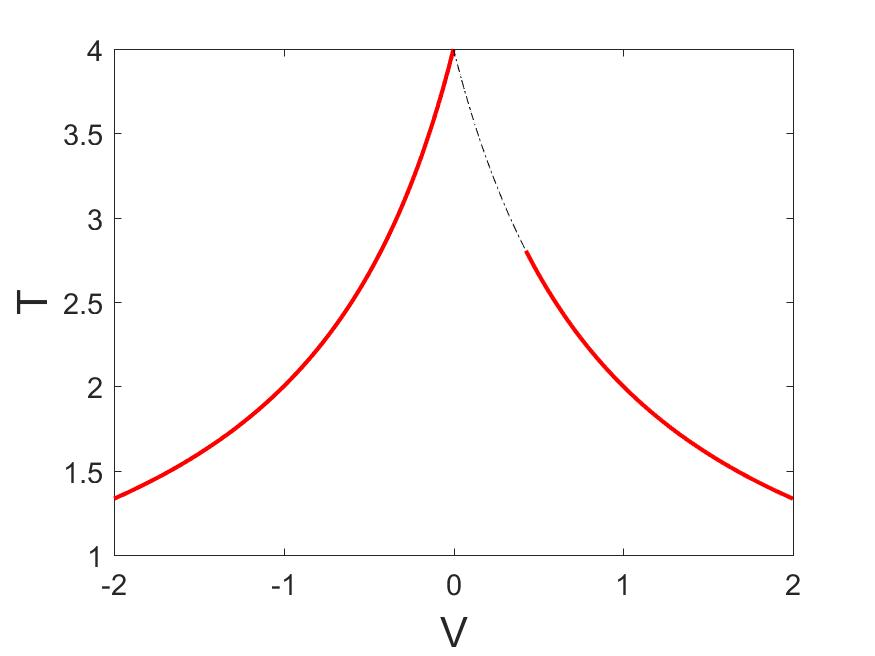
\includegraphics[width=\linewidth]{intro/T_equil.jpg}
 \caption{$V$ vs. $T$}
 \label{fig:Tequil}
\end{subfigure}%
\begin{subfigure}{.5\textwidth}
 \centering
 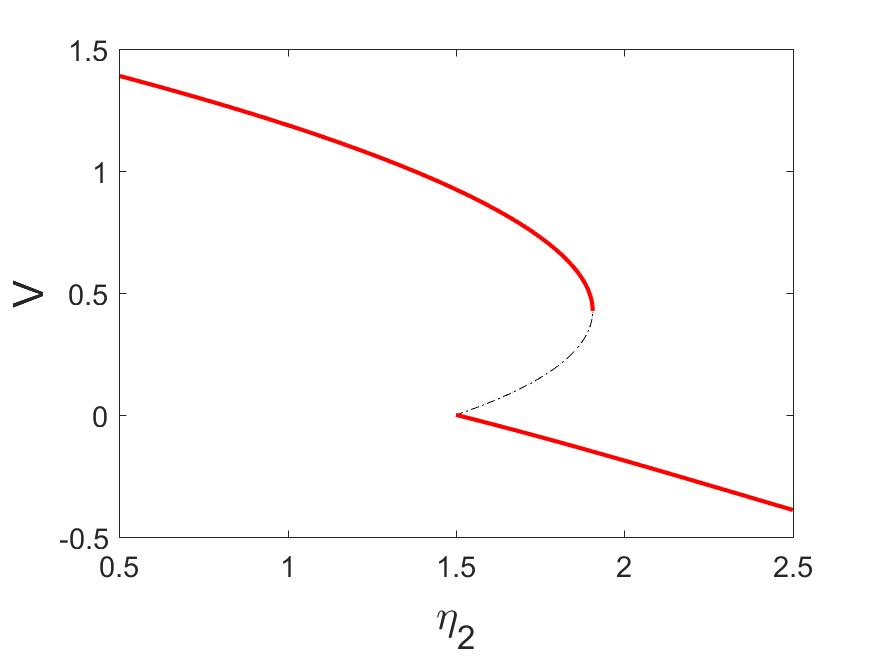
\includegraphics[width=\linewidth]{intro/V_bif.jpg}
 \caption{$\eta_2$ vs. $V$}
 \label{fig:Vbif}
\end{subfigure}
\caption{The equilibria of the non-dimensionalized system \eqref{eq:basic_stommel}. Parameters values are $\eta_1=4$ and $\eta_3=.375$. We see non-smooth behavior happening in both plots when $V=0$. The red line indicates a stable branch where the dashed dotted line is for an unstable branch.}
\label{fig:systemequil}
\end{figure}

As shown in figure~\ref{fig:systemequil}, the equilibrium curves reveal much about the dynamics. In (a) the graph of the equilibria for $V$ vs. $T$ shows non-smooth behavior occurring at $V=0$ and in (b) the two types of bifurcation appear clearly in the graph of equilibria for $\eta_2$ vs. $V$. In this plot, both the upper and lower branches of the equilibrium are stable with the middle branch being unstable. The stable branches relate to which variable is dominate. For the lower branch, we call this the halcine branch, and the upper branch the thermal branch. The location of the non-smooth bifurcation is found analytically, $({\eta_2}_{ns}V_{ns},T_{ns})=(\eta_1\eta_3,0,\eta_1)$, and the smooth bifurcation, $({\eta_2}_{\text{smooth}},V_{\text{smooth}},T_{\text{smooth}})$, is the only real solution to a cubic polynomial. The smoothness of each bifurcation is apparent and arise from the absolute value term in the defining dynamics of \eqref{eq:basic_stommel}, which is non-smooth only at $V=0$.

\begin{figure}[H]
\centering
\begin{subfigure}{.5\textwidth}
 \centering
 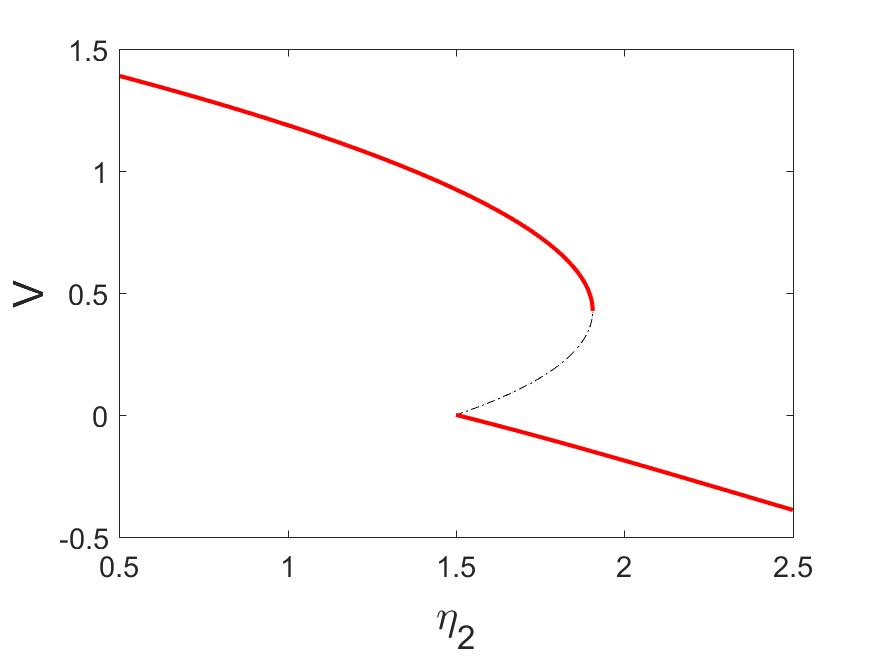
\includegraphics[width=\linewidth]{intro/V_bif.jpg}
 \caption{$\eta_3=.375$}
\end{subfigure}%
\begin{subfigure}{.5\textwidth}
 \centering
 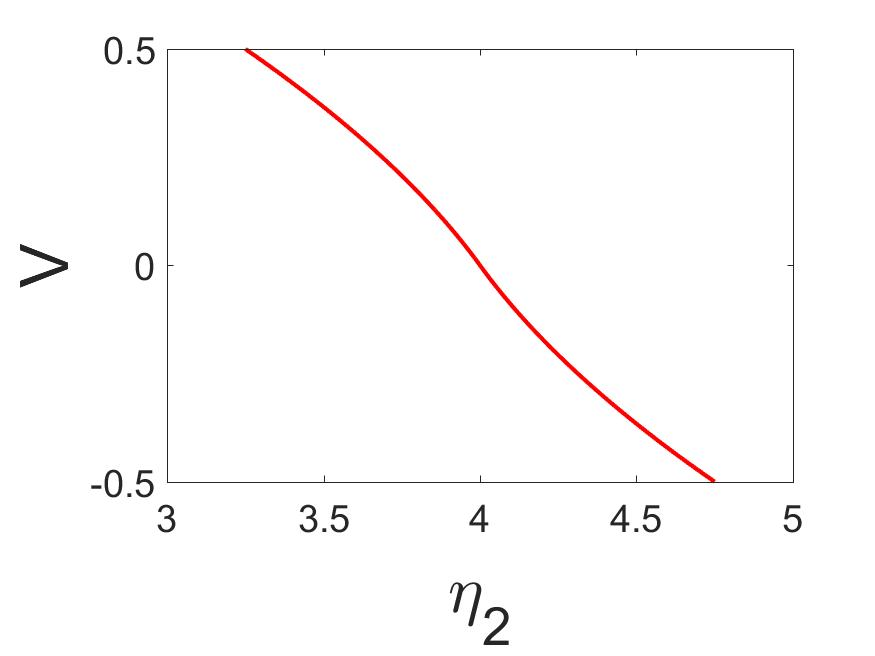
\includegraphics[width=\linewidth]{intro/V_bif_collapse.jpg}
 \caption{$\eta_3=1$}
\end{subfigure}
\begin{subfigure}{.5\textwidth}
 \centering
 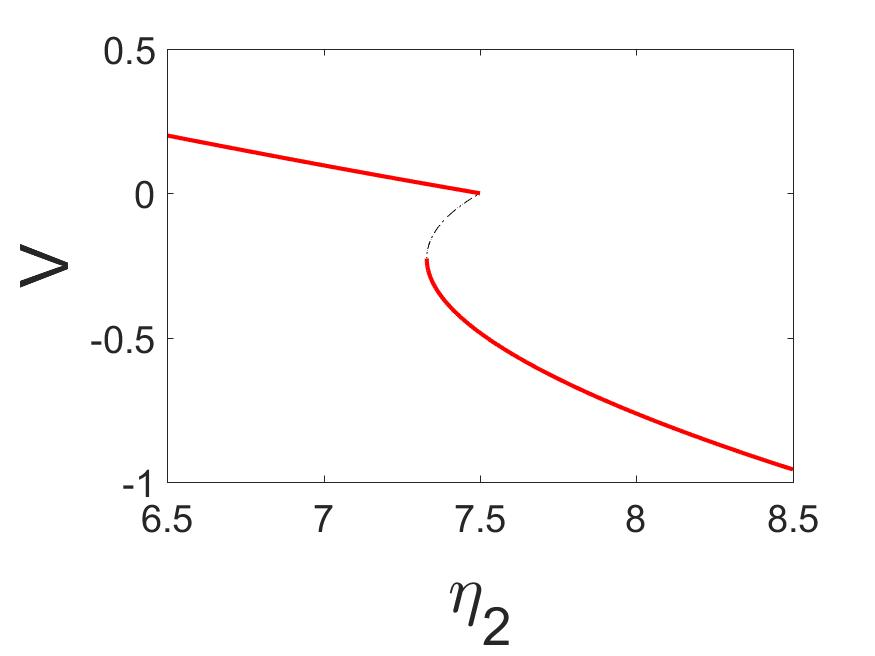
\includegraphics[width=\linewidth]{intro/V_bif_reverse.jpg}
 \caption{$\eta_3=1.875$}
\end{subfigure}
\caption{The choice in $\eta_3$ dictates the orientation of the problem, in each plot we have fixed $\eta_1=4$. The case for $\eta_3=1$ is special due to the two bifurcations overlapping and the unstable equilibrium vanishing.}
\label{fig:Stommel_bif_plots}
\end{figure}

Much is known about the Stommel model in the case where $\eta_2$ is fixed to be a constant value throughout the analysis but realistically this is not the case. In \cite{rahmstorf2000thermohaline}, this parameter is described as the influx of freshwater into the Atlantic and the changing nature of $\eta_2$ is justified by a positive feedback loop for salinity that drives the THC to move high-salinity water towards deep oceans. This loop causes the abrupt smooth bifurcation but then afterwards, a salinity deficit causes the parameter to decrease back towards the non-smooth bifurcation.

This type of behavior is known as hysteresis, where there is some bi-stability region that the solution cycles through and hits both states of the equilibria. A similar analysis to the Stommel model's hysteresis can be found in \cite{roberts2017relaxation}. The phenomenon of hysteresis appears in many physical systems, for example \cite{jung1990scaling}, \cite{hohl1995scaling} or \cite{joshi2005dynamical}. The smooth component of the hysteresis curve has been studied in a reduced one dimensional model, see \cite{zhu2015tipping}, we provide the other half of the analysis for the non-smooth component here.

\section*{Slowly Varying Tipping}
A system with a parameter known to cause a bifurcation will no longer admit a bifurcation in the standard sense when there is slow variation. Instead, these conditions give rise to a smooth but rapid change in the system's equilibria and where this occurs is called a tipping point.

A tipping point is a point that causes an abrupt smooth transition in dynamical behavior as the system moves into a qualitatively different state. The idea being that some positive feedback pushes change towards a different state once a critical point has been passed, for example with biological systems seen in \cite{angeli2004detection}. These are known to be caused by small changes in one or more parameters in the system. An analysis that lays the theoretic backing of slow varying tipping with algebraic bifurcations is found in \cite{haberman1979slowly}.

Tipping points have been discovered to occur in a wide variety of systems and have become a big staple in the study of areas like catastrophe theory and dynamical systems. They aid in predicting the future of a system and even could be a warning for irreversible change like in the case of the Stommel model. A tipping point thus shares similar characteristics of a bifurcation and typically occurs close to the standard bifurcation location.

An important paper that we extend the results of is \cite{zhu2015tipping} where work was done on the system

\begin{equation}\label{eq:intro_Zhueq}
\begin{aligned}
\dot{x} =& Da + k_0 +k_1 x + k_2 x^2,\\
\dot{a} =& -\epsilon,
\end{aligned}
\end{equation}

where $\mu\ll 1$. This system is a slowly varying quadratic differential equation containing a smooth saddle-node bifurcation and appears in many physical problems like \cite{erneux1989jump}. A major result from \cite{zhu2015tipping} is that the solution and tipping point for \eqref{eq:intro_Zhueq} have the form

\begin{equation}\label{eq:intro_Zhuairy}
x\sim \frac{1}{|k_2|}\left(\frac{k_1}{2}+\left(\frac{D|k_2|}{\epsilon}\right)^{1/3}\right)\frac{Ai'\left([D|k_2|\epsilon]^{-2/3}\left(\frac{k_1^2}{4}+k_0|k_2|+D|k_2|a\right)\right)}{Ai\left([D|k_2|\epsilon]^{-2/3}\left(\frac{k_1^2}{4}+k_0|k_2|+D|k_2|a\right)\right)}
\end{equation}

\begin{equation}\label{eq:intro_Zhuresult}
a_{\text{tip}}=(D|k_2|)^{-1/3}a_{\text{Airy}}-\frac{a_s}{D}\quad \text{for} \quad a_s = k_0+\frac{k_1^2}{4|k_2|},
\end{equation}

with $Ai(\cdot)$ being the Airy function and $a_{\text{Airy}}=\epsilon^{2/3}\cdot(-2.33810\ldots)$ corresponding to the first zero of the Airy function. The tipping found in \eqref{eq:intro_Zhuresult} is a recurring tool for the work presented in this paper, even though we deal with a version of \eqref{eq:intro_Zhueq} that has a non-smooth bifurcation.

\begin{figure}[H]
\centering
\begin{subfigure}{.5\textwidth}
 \centering
 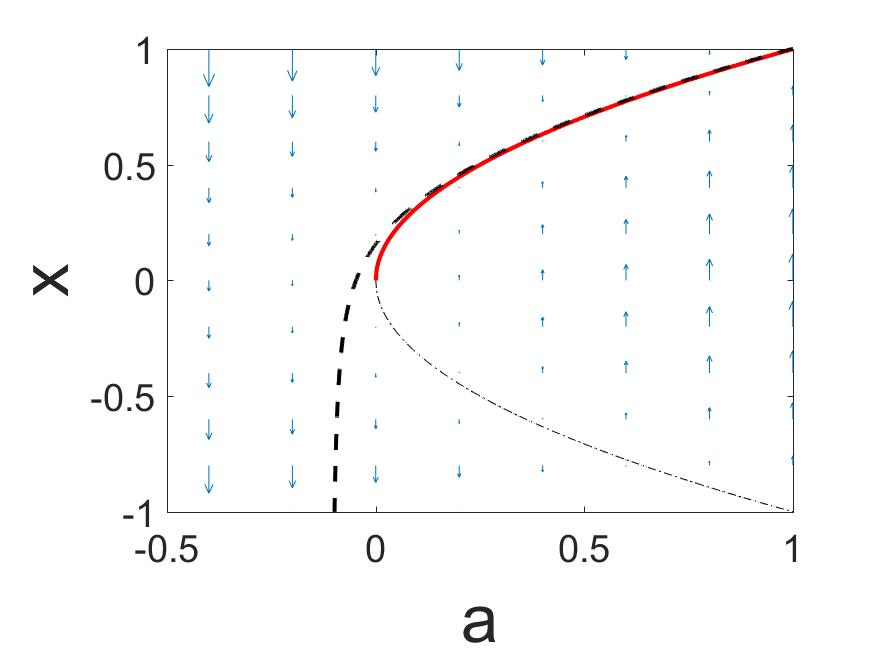
\includegraphics[width=\linewidth]{intro/saddlenode_tipping.jpg}
 \caption{}
\end{subfigure}%
\begin{subfigure}{.5\textwidth}
 \centering
 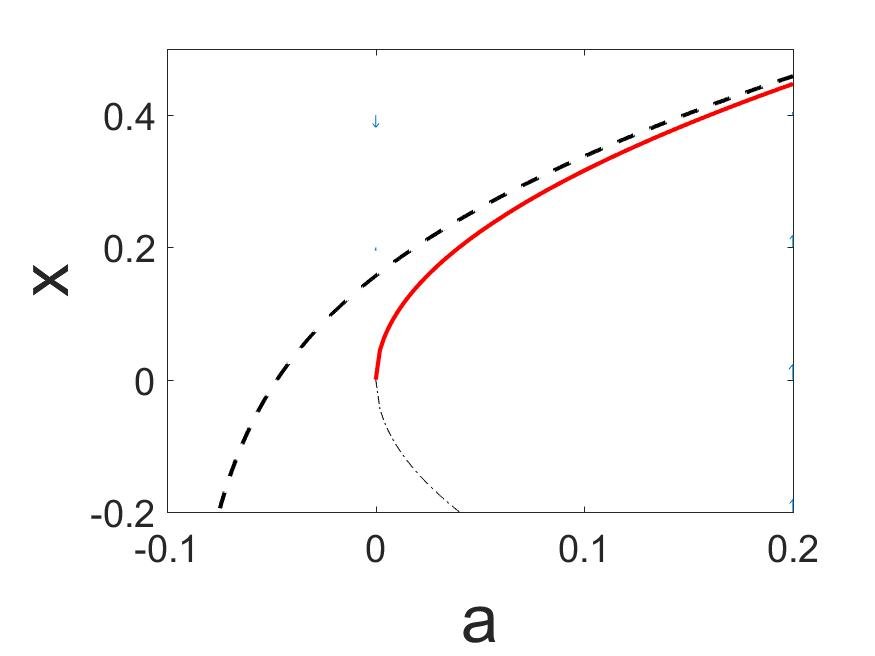
\includegraphics[width=\linewidth]{intro/saddlenode_tipping_zoom.jpg}
 \caption{}
\end{subfigure}
\caption{An example of tipping occurring in the saddle-node around the saddle-node bifurcation.}
\label{fig:intro_tipping}
\end{figure}


In figure~\ref{fig:intro_tipping} we show a numerical solution to the simple saddle-node system with tipping \eqref{eq:intro_Zhueq}. Here we have $D=1$, $k_0=k_1=0$ and $k_2=-1$ which is the model in \eqref{eq:intro_saddlenode} we saw earlier. The solution follows closely to the stable branch even after the bifurcation would have occurred, which is indicative of this delayed-typed behavior.


The task of finding where tipping occurs depends on the situation, but in general the approach is to search for when a solution to a problem fails or becomes uncontrollable. This happens when the solution fails to be real or when an exponential term grows too quickly, both of which we see throughout this paper.
